\section{Configuration Details}
\label{app:configuration}

The canonical configuration and schedule inputs are under \texttt{configs/}.
The main report's C1-C8 matrix lists the tested read concern, write concern,
causal-session setting, and target properties. Additional deployment defaults
are:

\begin{itemize}
\item replica-set name: \texttt{rs0}; three data-bearing members;
\item database port inside each container: 27017;
\item default host ports: 27017, 27018, and 27019;
\item client subnet: 172.19.0.0/16; replica subnet: 172.20.0.0/16;
\item operation deadlines, retry policy, and preconditions: \path{docs/experimental-protocol.md}.
\end{itemize}

The prediction targets are stored in \texttt{configs/predictions.json}; the
runner, schema, campaign, and schedule contracts are versioned alongside it.
Reported settings come from those configuration files and the campaign
manifests, not from a mutable setup snapshot.

\section{Installation and Reproduction Commands}
\label{app:install}

Run from the repository root in a clean checkout. \texttt{make setup} verifies
the local toolchain and initializes the Docker Compose replica set. The
campaign commands require the Docker services. Offline analysis and report
building use saved artifacts and remain development commands outside the
runtime archive. Smoke and pilot are optional diagnostics before a new campaign;
they are not part of the final result set.

\begin{verbatim}
python3 -m pip install -r requirements-dev.txt
make setup
make smoke
make pilot
make experiment
make rq2
make test
make check-docs
make check-schemas
make check-runner-isolation
make analyse
make rq4-analyse
make submission
make check-submission-artifacts
make check-release-ready
\end{verbatim}

Smoke and pilot outputs are not pooled into the main campaign results. The
campaign manifest records status, source provenance, software versions, and
image digest. Analysis validates and recomputes outcomes from canonical raw
histories before building the report. The release-readiness check also
requires complete team metadata.

\begin{figure}[ht]
\centering
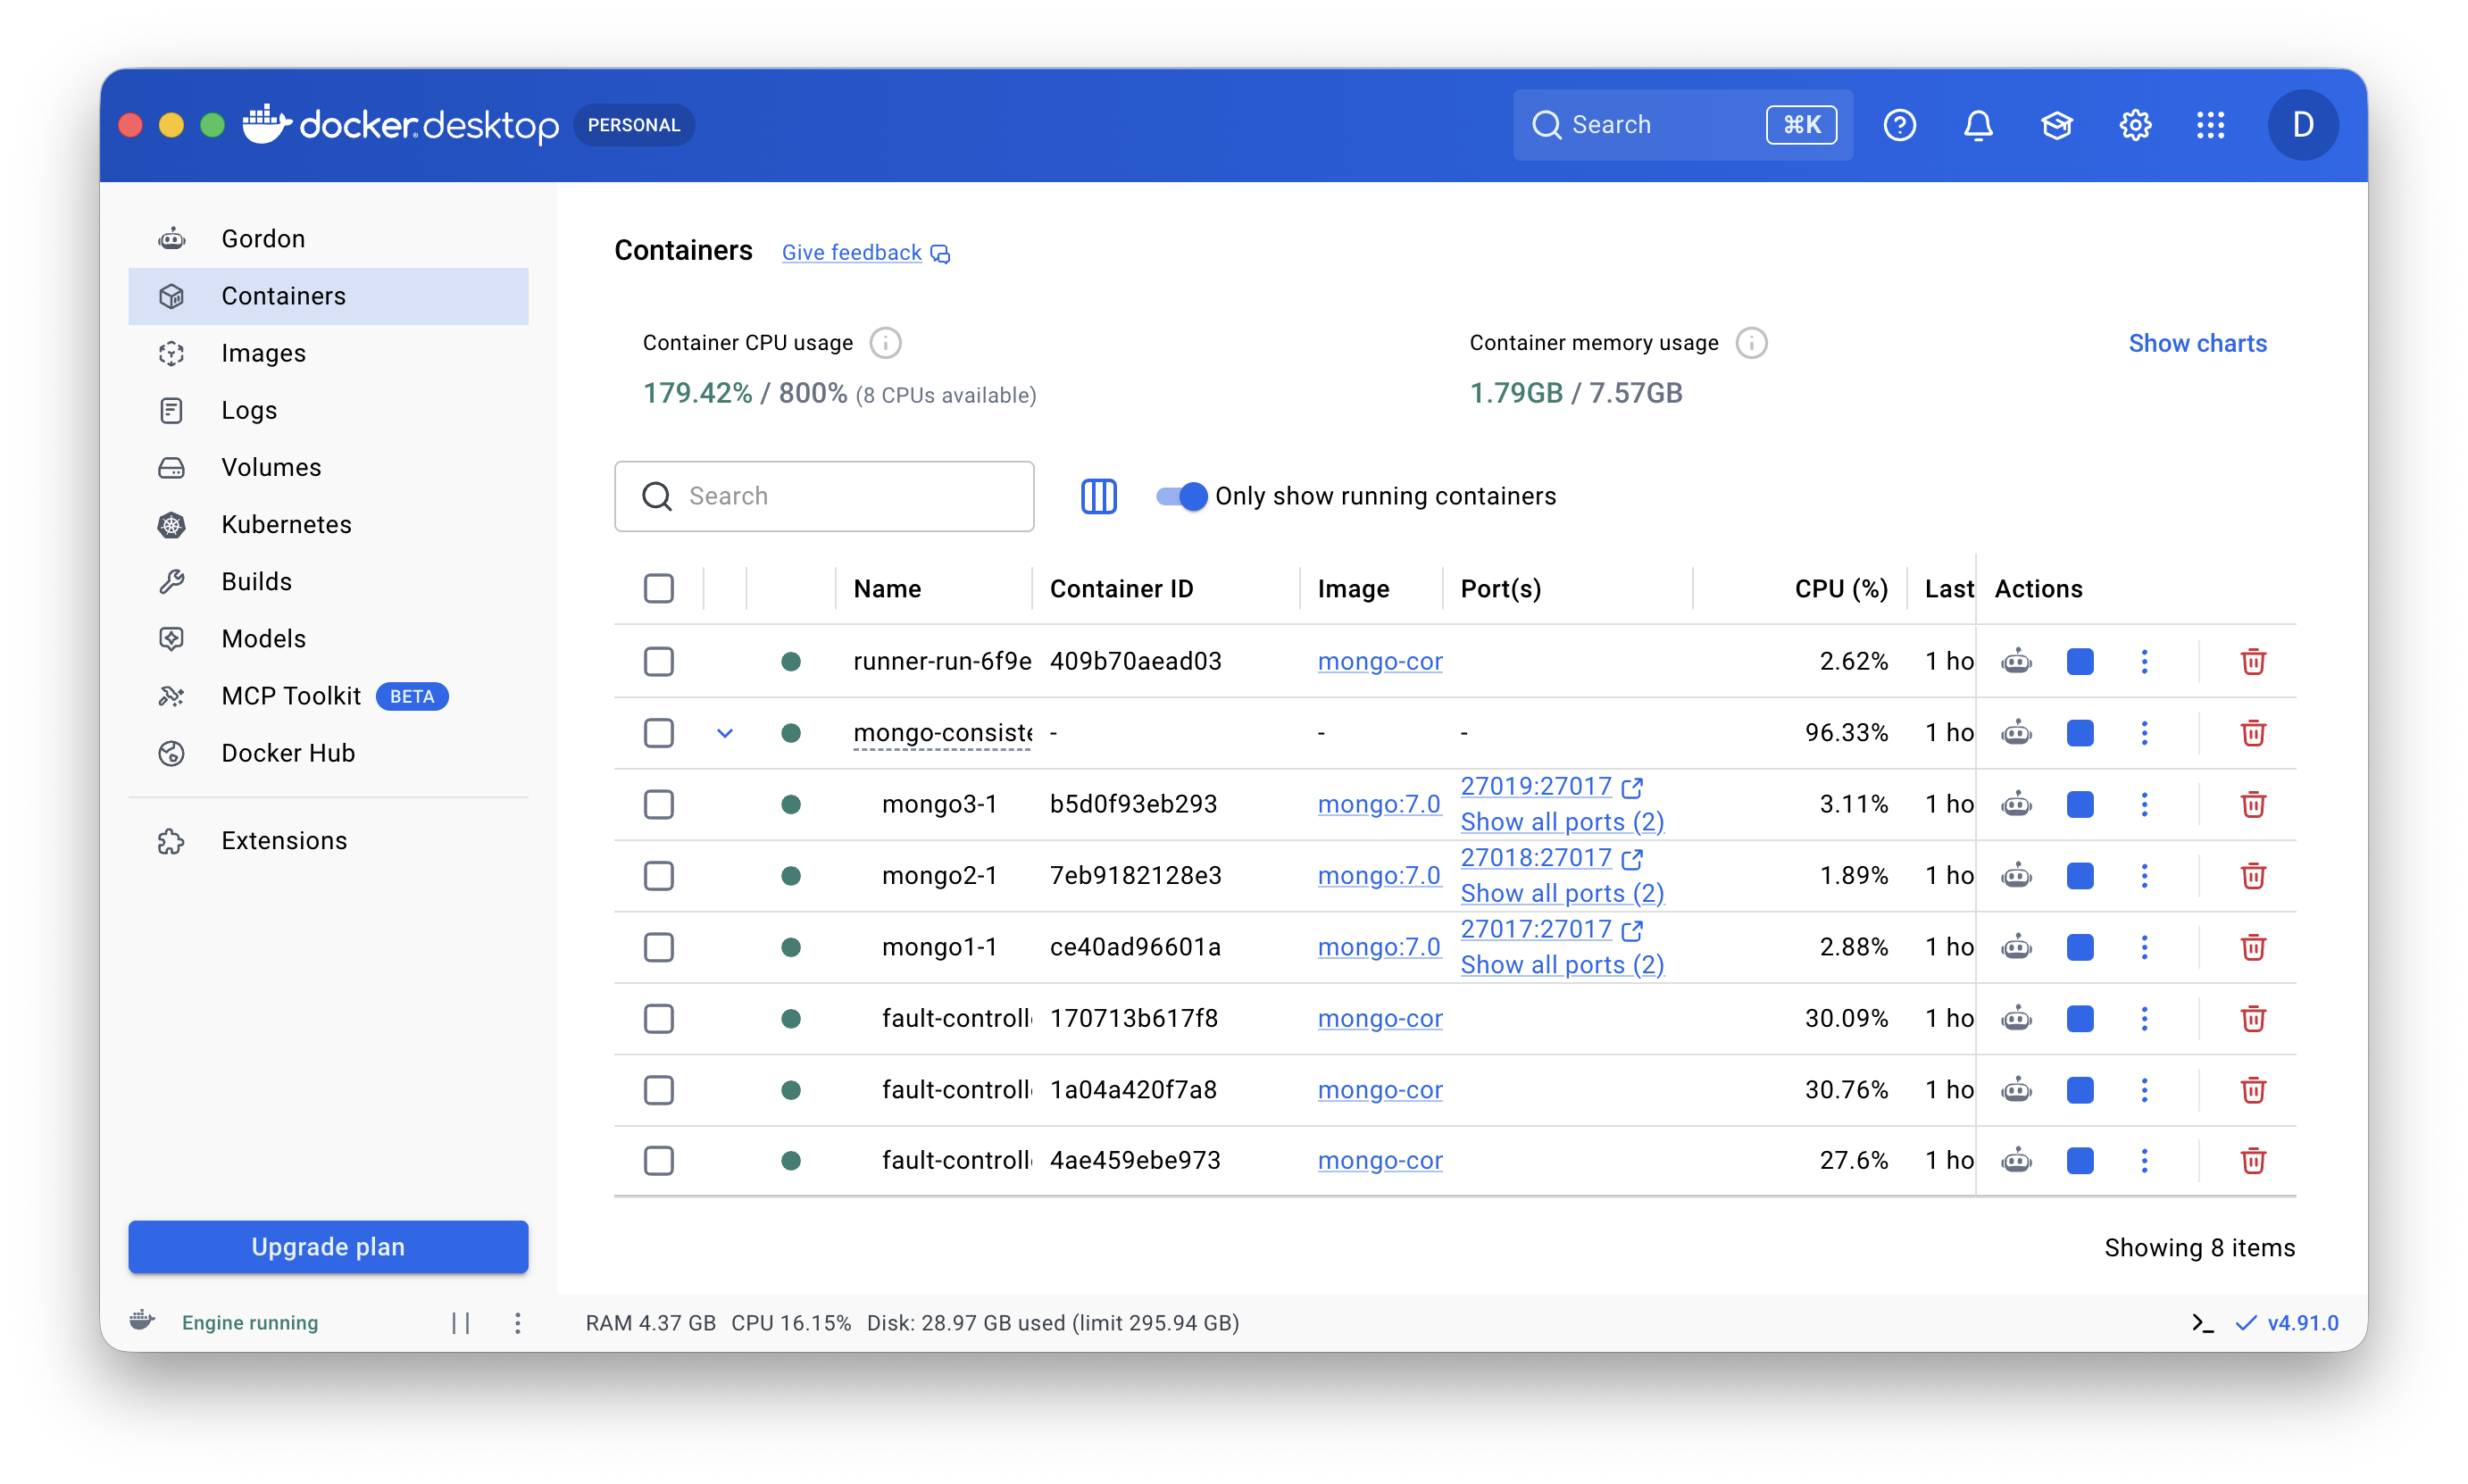
\includegraphics[width=0.88\linewidth]{submission/evidence/docker-desktop-running.png}
\caption{Docker Desktop showing the runner, MongoDB members, and fault controllers used for the recorded setup.}
\label{fig:docker-desktop-running}
\end{figure}
\FloatBarrier

\section{Full Result Matrices and Audit Data}
\label{app:full-results}

Machine-readable results are under \texttt{results/summary/}; canonical
histories and manifests are under \texttt{results/raw/}. The fault episode table
records fault application, election, and recovery at the episode level. The
completion analysis recomputes client-visible violation, observed definitive
completion, and separate all-attempt and resolved critical-operation p50/p95
latency from the campaign histories and writes
\texttt{results/summary/rq4/metrics.csv}, \texttt{contrasts.csv}, and
\texttt{fault\_deltas.csv}.

\subsection{Full fault and configuration matrices}

\begin{table}[ht]
\centering
\small
\setlength{\tabcolsep}{3pt}
\caption{Configuration campaign outcomes by property. G marks a prediction target and N a descriptive cell. P, V, U, I, PM, and HE denote PASS, VIOLATION, UNAVAILABLE, INDETERMINATE, PRECONDITION\_MISS, and HARNESS\_ERROR. Only P and V enter the decidable comparison.}
\label{tab:prediction-observation}
\begin{tabular}{@{}l*{4}{p{0.19\textwidth}}@{}}
\toprule
Config. & RYW & MR & MW & WFR \\
\midrule
\RQOnePredictionObservationRows
\bottomrule
\end{tabular}
\end{table}

The main report uses the fault-level summary in Table~\ref{tab:fault-summary}.
These tables retain the configuration-property rows, p99 values, rollback
counts, and episode timing used to derive that summary.

{\footnotesize
\setlength{\tabcolsep}{3pt}
\begin{longtable}{@{}l l l c r p{0.20\textwidth} c@{}}
\caption{Target and outcomes by fault, configuration, and property.}
\label{tab:rq2-outcomes}\\
\toprule
Fault & Config & Property & Target & $n$ & P/V/U/I/PM/HE & Ops S/A \\
\midrule
\endfirsthead
\caption[]{Target and outcomes by fault, configuration, and property (continued).}\\
\toprule
Fault & Config & Property & Target & $n$ & P/V/U/I/PM/HE & Ops S/A \\
\midrule
\endhead
\midrule
\multicolumn{7}{r}{Continued on next page}\\
\endfoot
\bottomrule
\endlastfoot
\RQTwoOutcomeRows
\end{longtable}
}

{\footnotesize
\setlength{\tabcolsep}{3pt}
\begin{longtable}{@{}l l l r r r r@{}}
\caption{Latency and acknowledged-write rollback by fault, configuration, and property.}
\label{tab:rq2-latency-rollback}\\
\toprule
Fault & Config & Property & All-attempt latency p50/p95/p99 (ms) & Ack writes & Checked/rolled back & Rollback (\%) \\
\midrule
\endfirsthead
\caption[]{Latency and acknowledged-write rollback (continued).}\\
\toprule
Fault & Config & Property & All-attempt latency p50/p95/p99 (ms) & Ack writes & Checked/rolled back & Rollback (\%) \\
\midrule
\endhead
\midrule
\multicolumn{7}{r}{Continued on next page}\\
\endfoot
\bottomrule
\endlastfoot
\RQTwoMetricRows
\end{longtable}
}

\begin{longtable}{@{}lrrrrrr@{}}
\caption{Election and recovery by fault episode. Times are p50 seconds.}
\label{tab:rq2-episodes}\\
\toprule
Fault & Episodes & Applied & Elections & Election p50 & Converged & Recovery p50 \\
\midrule
\RQTwoEpisodeRows
\bottomrule
\end{longtable}

\subsection{Matched-pair audit}
\label{app:matched-pair-audit}

The mechanism analysis compares control-valid pairs. This appendix retains
the pair and signature counts. Trial IDs, raw histories, and complete SHA-256
values remain in
\texttt{results/analysis/rq3/summary.json} and
\texttt{results/analysis/rq3/selection-manifest.json}.

\begin{table}[ht]
\centering
\small
\caption{Matched-pair control counts.}
\label{tab:rq3-pair-controls}
\begin{tabular}{@{}l p{0.40\linewidth} r r r@{}}
\toprule
Contrast & Factor & Planned & Valid & Invalid \\
\midrule
M1 & C5 versus C6, causal session & 8 & 8 & 0 \\
M2 & C8 versus C5, read concern & 8 & 8 & 0 \\
M3 & C3 versus C6, write concern & 8 & 8 & 0 \\
\bottomrule
\end{tabular}
\end{table}

\begin{table}[ht]
\centering
\small
\caption{Signature counts from the eight valid pairs in each contrast.}
\label{tab:rq3-signature-counts}
\begin{tabular}{@{}l p{0.78\linewidth}@{}}
\toprule
Contrast & Observed signatures \\
\midrule
M1 & C5 stale read: 8/8; C6 causal bound present: 8/8; C6 read unavailable: 8/8 \\
M2 & C8 local v1: 8/8; C5 majority v0: 8/8; C8 WFR violations: 5/8 and indeterminate: 3/8; C5 WFR passes: 4/8 and indeterminate: 4/8; W2 present on every final member in both arms: 8/8 \\
M3 & C3 W1 acknowledged: 8/8; W1 absent from W2's atomic pre-image: 8/8; C3 MW violations: 8/8; C6 majority W1 timed out: 8/8; C6 MW indeterminate: 8/8 \\
\bottomrule
\end{tabular}
\end{table}
\FloatBarrier

\subsection{RQ4 detailed metrics}
\label{app:rq4-details}

The main text reports the balanced partition signatures and one-factor
contrasts. This table retains the selected C5/C6 cells with separate
all-attempt and resolved latency samples.

\begin{table}[ht]
\centering
\small
\setlength{\tabcolsep}{3pt}
\caption{RQ4 selected C5/C6 metrics; counts, observed completion, and separate latency samples.}
\label{tab:rq4-selected-metrics}
\begin{tabular}{@{}l l l r r r r@{}}
\toprule
Scenario & Config & Property & P/V/U/I & $D$ & All-attempt p50/p95 (ms) & Resolved p50/p95 (ms) \\
\midrule
\RQFourSelectedRows
\bottomrule
\end{tabular}
\end{table}

\maybefigure[fig:rq4-outcomes-partition]{submission/figures/rq4_outcomes_partition.pdf}{RQ4 paired C1/C6 RYW and MW signature outcomes under the RQ2 partition.}
\maybefigure[fig:rq4-c5-c6]{submission/figures/rq4_c5_c6_contrast.pdf}{RQ4 C5/C6 one-factor contrast under normal and RQ1 fault scenarios.}


\subsection{Additional figures}

The following figures are retained for audit and interpretation. They are
descriptive views of the measured histories, not additional experiments.
They were exported as vector PDFs with Matplotlib 3.11.2 and SciencePlots
2.2.2~\cite{scienceplots}. Plot generation reads the saved histories and does
not write report sections.

\maybefigure[fig:factorial-interactions]{submission/figures/factorial-interactions.pdf}{Descriptive factorial contrasts from adversarial configuration histories. RC, WC, and CS denote read concern, write concern, and causal session; interaction columns compare combinations of these factors. Values are signed contrasts for the checked metric, not causal effect estimates. NA means the contrast could not be calculated.}
\maybefigure[fig:outcome-heatmap]{submission/figures/outcome-heatmap.pdf}{Adversarial configuration outcome matrix without prediction borders. Each cell gives violations over decidable histories; unresolved cells contain no decidable history. This view repeats Figure~\ref{fig:prediction-observation} for audit rather than adding a new experiment.}
\maybefigure[fig:latency]{submission/figures/latency.pdf}{Operation latency quantiles for normal controls and adversarial configuration histories. The vertical scale is logarithmic when timings are available. The plot includes all timed subject operations, including failed attempts, and excludes pilot histories.}
\FloatBarrier
